\documentclass[12pt,a4paper]{report}
\usepackage{amssymb,amsthm,amsmath,amscd}
\usepackage{latexsym}
\usepackage{enumerate}
\usepackage[german]{babel}
\usepackage{verbatim}
\usepackage[utf8]{inputenc}
\usepackage{hyperref}
\usepackage{graphicx}



\begin{document}
% ---------------

\begin{titlepage}
	\begin{center}
		
		\vspace*{1.0cm}
		\huge
		\textsc{\bf{PS Netze und Verteilte Systeme}}
		
		\vspace*{4.0cm}
		\textsc{
			\normalsize{eingereicht von} \\[0.5\baselineskip]
			{\large Baumgartner Dominik}
		}
		
		\vspace*{3.0cm}
		\textsc{
			\normalsize{Gruppe 1(13:00)}
		}
		
	\end{center}
	
\end{titlepage}

\ \\
\textbf{Aufgabe 17:}
\\
\\
Was ist Zweck und Funktionsweise des Address Resolution Protocol (ARP) für IPv4? 
\\
\\
Zweck: ARP ist ein Netzwerkprotokoll, das zu einer Netzwerkadresse (IP-Adresse) die physikalische Adresse (MAC-Adresse) ermittelt und diese Zuordnung gegebenenfalls in einer ARP-Tabellen der beteiligten Rechner hinterlegt\\
Funktionsweise: Es wird eine ARP-Anforderung mit der MAC-Adresse und der IP-Adresse des anfragenden Computers als Senderadresse und der IP-Adresse des gesuchten Computers als Empfänger-IP-Adresse an alle Computer des lokalen Netzwerkes gesendet. Als Empfänger MAC-Adresse wird ff-ff-ff-ff-ff-ff gesendet (MAC-Broadcast an alle Systeme im Netzwerk). Empfängt ein Computer nun solch ein Paket, sieht er nach ob seine Adresse die Empfängeradresse dieses Paketes ist. Wenn dem so ist, antwortet er mit dem zurücksenden seiner IP- und MAC-Adresse an die MAC-Adresse
des Anfordernden Gerätes (ARP-Antwort). Nach Empfangen der Antwort, werden die übermittelten Adressen in seine ARP-Tabelle eingetragen.\\
\\
\textbf{Aufgabe 19:}
\\
\\
 Welche Vor- und Nachteile hat es, wenn Router auf Broadcast ARP Nachrichten für
 Adressen außerhalb des lokalen Subnets antworten würden.
\\
\\

\textbf{Aufgabe 20:}
\\
\\
Erklären Sie die Struktur einer IPv4 Adresse. Welche Adress-Klassen gibt es?
Welche Bereiche sind für spezielle Zwecke reserviert? Was versteht man unter
„Classless Interdomain Routing (CIDR)"?
\\
\\
IPv4 benutzt 32-Bit-Adressen, daher können in einem Netz maximal $2^{32}$ Adressen vergeben werden.
IPv4-Adressen werden üblicherweise dezimal in vier Blöcken geschrieben. Jeder Block repräsentiert 8 Bit $\Rightarrow$ somit ergibt sich für jeden Block ein Wertebereich von 0 bis 255. 
Eine IP-Adresse besteht aus einem Netzanteil und einem Hostanteil. Der Netzanteil identifiziert ein Teilnetz, der Hostanteil identifiziert ein Gerät (Host) innerhalb eines Teilnetzes.
\\
\\
Classless Inter-Domain Routing: Dies ist ein Verfahren zur effizienteren Nutzung der $2^{32}$ möglichen Adressen von IPv4. Bei CIDR entfällt die feste Zuordnung einer IP-Adresse zu einer Netzklasse. Hierbei wird eine neue Notation eingeführt, sog. Suffixe. Ein Suffix gibt die Anzahl an 1er Bits in der Netzmasek an. BSP: 192.168.0.0/255.255.0.0 wird geschrieben als: 192.168.0.0/16. Diese Schreibweise ist wesentlich kürzer und genauso eindeutig.
Berechnung (Bsp. von Wikipedia): 
Subnetzmaske: 11111111.11111111.11111111.1111\textbf{0000} $\Rightarrow$ mit diesen vier 0er Stellen lassen sich 16 verschieden Zahlen darstellen. Minus Netwerkadresse und Broadcastadresse ergibt dies 14 versch. IPv4 Adressen
\\
\\
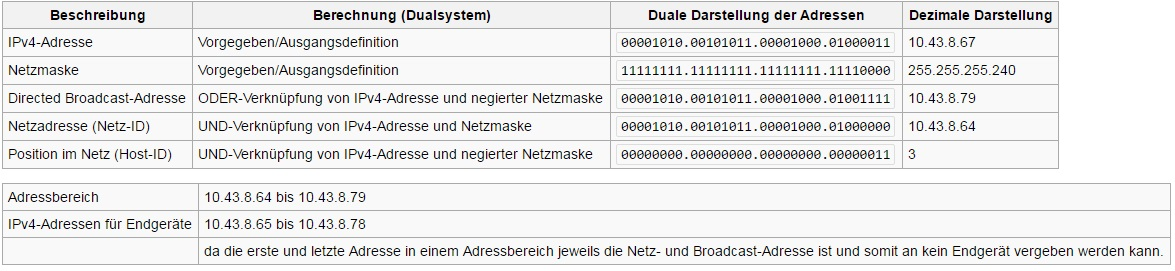
\includegraphics[width = 17cm, height = 4cm]{bsp-cidr.jpg}
\ \\
Klasse A:\\
Die Submaske ist in der Klasse A immer 255.0.0.0, über die Subnetzmaske wird definiert welcher Teil der IP-Adresse die NetzwerkID und was die \\HostID ist.\\
Bsp: zu Klasse A:\\
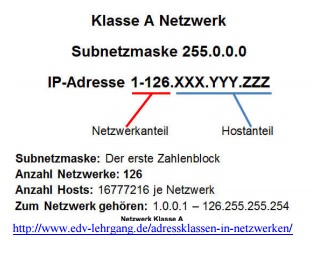
\includegraphics[width = 7cm, height = 6cm]{classa.jpg}
\\
Besonderheit im Netzwerk 0 – 127:
Die Netzwerke 0 und 127 sind für spezielle Netzwerke mit besonderen Eigenschaften
reserviert. Beispielsweise ist die Netzwerkadresse 127.0.0.1 immer die IP-Adresse des lokalen
Rechners und wird auch Loopback-Adresse genannt. Daher können die Netzwerke 0 und 127
nicht zu den verwendbaren Klasse A Netzwerken gezählt werden.\\
Klasse B:\\
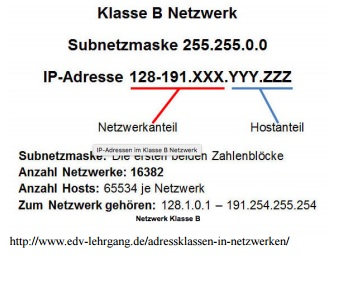
\includegraphics[width = 7cm, height = 6cm]{classb.jpg}
\\
Klasse C:\\
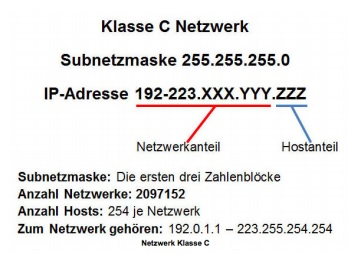
\includegraphics[width = 7cm, height = 6cm]{classc.jpg}
\\
Klasse D und E:\\
Diese beiden Adressklassen sind besondere Netzwerkklassen.
D wird für Multicast adressen benötigt. E Netzwerk ist für Zukünftige Anwendungen
reserviert.\\
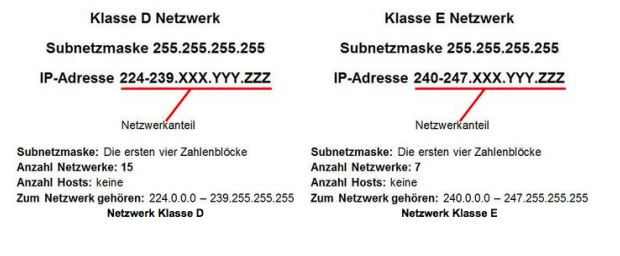
\includegraphics[width = 13cm, height = 5cm]{classde.jpg}
\newpage
\ \\
\textbf{Aufgabe 23:}
\\
\\
Wie funktioniert DHCPv4 und welche Vor- und Nachteile hat es?
\\
\\
DHCP bedeutet Dynamic Host Configuration Protocoll (Kommunikationsprotokoll). Es
ermöglicht Zuweisung von Netzwerkkonfiguration von Clients über den Server.\\
\\
DHCP-Server:\\
Der DHCP-Server wird als Hintergrundprozess gestartet und wartet auf UDP-Port 67 auf Client-Anfragen. In seiner Konfigurationsdatei befinden sich Informationen über den zu vergebenden Adresspool sowie zusätzliche Angaben über netzwerkrelevante Parameter.Es gibt drei verschiedene Betriebsmodi eines DHCP-Servers: manuelle, automatische und dynamische Zuordnung.\\
\textbf{manuell:} Hierbei werden am DHCP-Server die IP-Adressen bestimmten MAC-Adressen fest zugeordnet.\\
\textbf{automatisch:} Hier wird am DHCP-Server ein Bereich von IP-Adressen definiert und diese Adressen automatisch an die MAC-Adresse von neuen Clients zugewiesen. Diese Zuweisungen werden in einer Tabelle festgehalten.\\
\textbf{dynamisch:} Wie automatisch, nur dass der Server in seiner Konfigurationsdatei eine Angabe hat, wie lange eine IP-Adresse an einen Client "verliehen" werden darf.\\
\\
Vorteil:
\begin{itemize}
	\item IP-adressenverwaltung
	\item Zentralisierung und Konfiguration von Netzwerken
	\item Unterstützt BOOTP-Clients
	\item Unterstützung von lokalen und remote Clients
\end{itemize}
Nachteile:
\begin{itemize}
\item Keine guten Sicherheitsmechanismen auf Protokollebene
\item Wenn DCHP ausfällt bekommen neue Clients keine IP und bestehende können
Adressen nicht erneuern
\end{itemize}
% -------------
\end{document}
